\subsection{层次聚类介绍}
在最开始,每个数据点作为单独的群集开始,然后合并相邻的群集以形成树状结构。
简单来说,这可以被看作是自下而上的聚类方法。
层次聚类是一种强大的无监督学习算法,它通过创建数据的层次结构来对相似的数据进行分组。
该算法的优点在于能够帮助可视化和理解数据间的相似性。
此外,通过层次结构可以创建更详细的分组,并理解群组间的关系和层次结构。 \par

它主要应用于社交网络分析、客户细分、地理信息系统等领域。例如,在生物学中,它可以用于理解基因分析、物种分类和进化关系等。
总之,由于这种算法提供了基于数据相似性的分析,因此它对于识别数据的结构和模式、提取信息非常有用。 \par

通过测量数据之间的距离和聚类合并过程,可以获得有价值的信息。\par

\subsection{使用层次聚类对图像进行识别的效果分析}
\begin{figure}[H]
    \centering
    \subfigure[训练结果1]{
        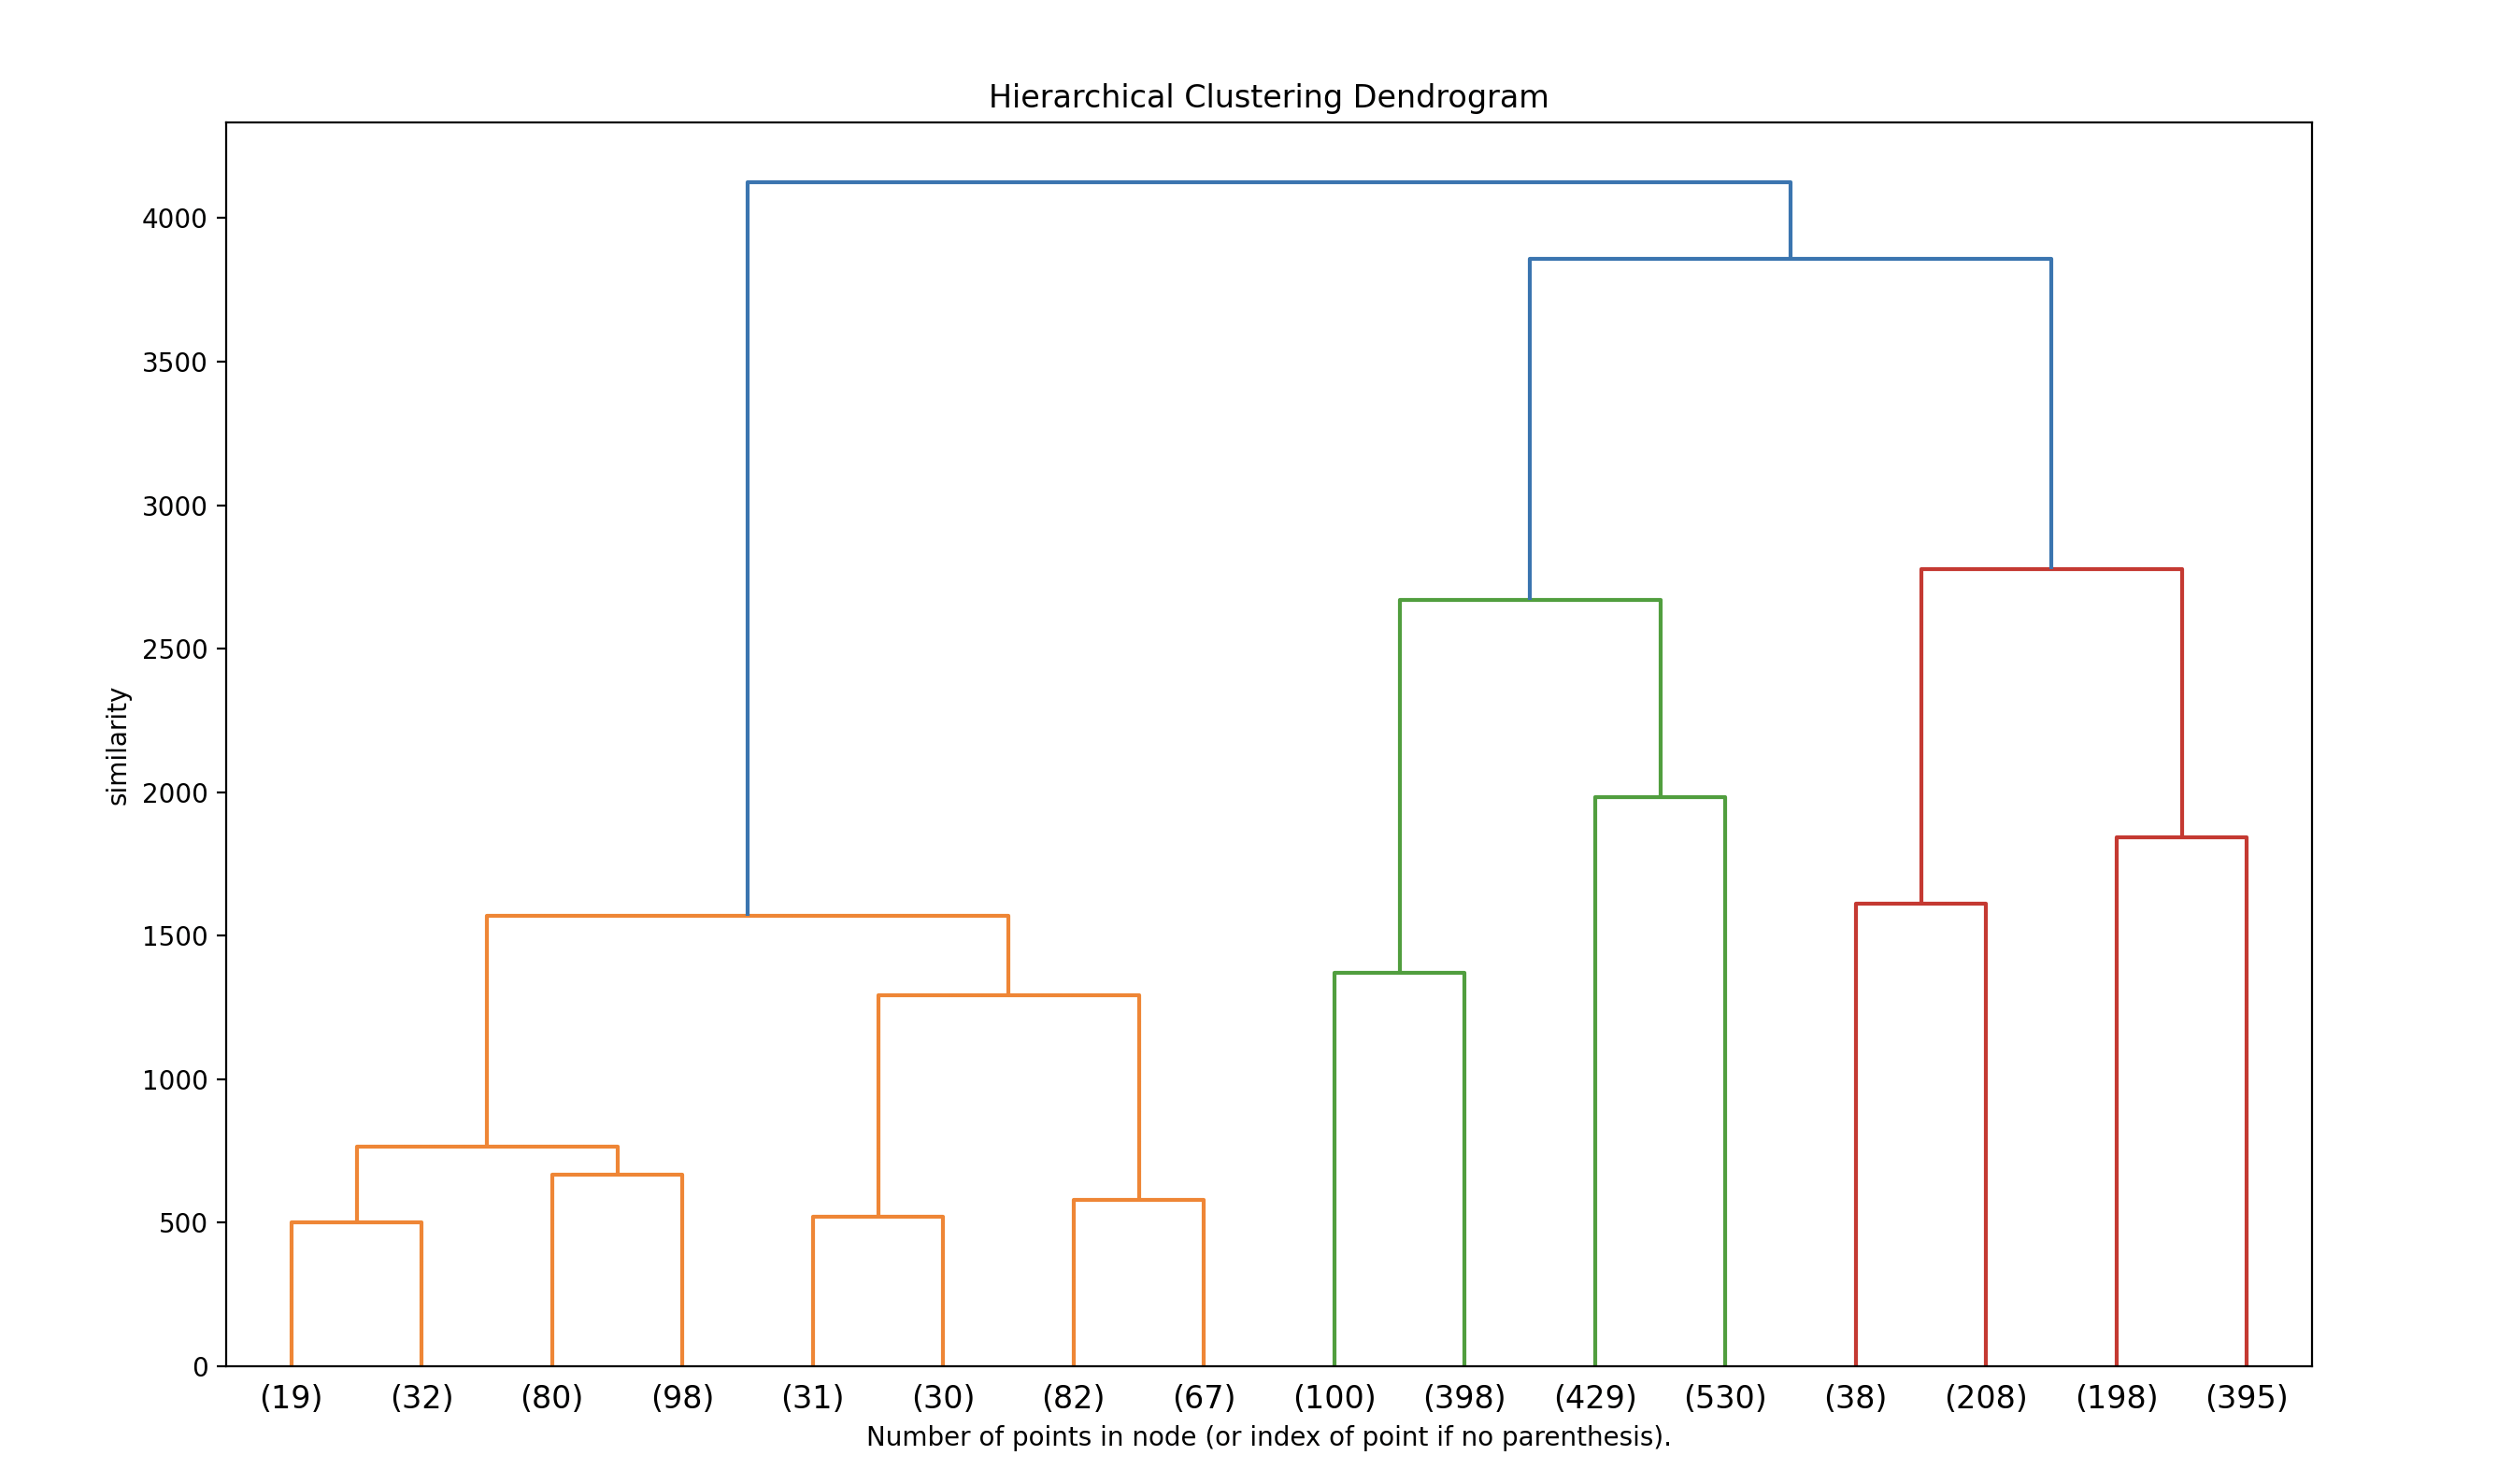
\includegraphics[width=7cm]{../../Hierarchical_Clustering/Hierarchical_Clustering_1.png}
    }\quad
    \subfigure[训练结果2]{
        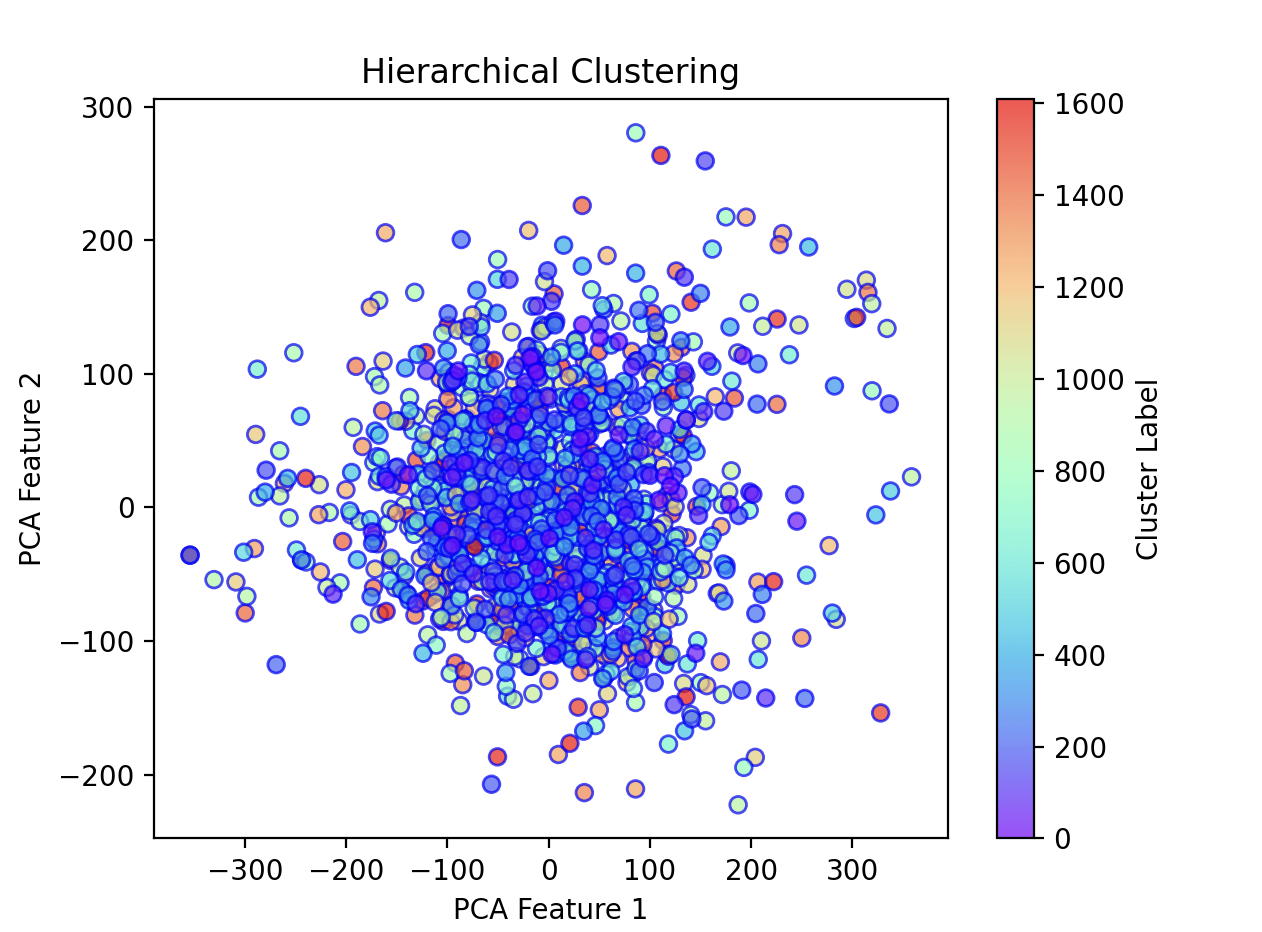
\includegraphics[width=7cm]{../../Hierarchical_Clustering/Hierarchical_Clustering_2.png}
}\end{figure}

数据集中的图像之间的差异在于车型和颜色。
层次聚类是将彼此相似的图像聚集在一起形成群集的过程,形成得越快的群集其相似性就越大。
为了便于理解,我们来看看树状图的黄色条形图,首先,X轴上的节点数,如19、32、80、98等,表示最初聚集在一起的群集中的图像数量。
这是最初聚集在一起的最相似的图像群集。
接下来,由19个图像组成的群集和由32个图像组成的群集在相似度数值500处形成了一个群集。
这意味着与其他群集相比,由19个图像组成的群集和由32个图像组成的群集更为相似(相似度数值为500),因此它们聚集在一起形成了下一个群集。
相似度数值越接近0,就越相似。通过这种层次化的方式,最终形成一个群集。在最开始群集的形成标准是车型和颜色中的哪一个,需要自主判断。